% !TEX root = ../report.tex
\section{Die Benutzeroberfläche}
\begin{Spacing}{\mylinespace}

Nachdem die Grundfunktionalität der Hauptkomponenten unseres Systems standen ging es nun daran eine einfache aber dennoch funktionale Benutzeroberfläche zu entwerfen. Da das \textit{XNA-Framework} von Haus aus auf \textit{Windows-Forms} zur Darstellung von Benutzeroberflächen setzt, beschlossen auch wir vorerst diese Variante zu nutzen. Hielten uns aber die Möglichkeit offen eventuell später auf das etwas modernere \textit{WPF}-System zu wechseln.
\\\\
Hauptanforderungen waren ein übersichtliches Design und ein einfaches Hinzufügen von neuen Funktionalitäten. Um diese Anforderungen zu erfüllen entschieden wir uns für eine schlichte Statusleiste am unteren Rand des Editor-Fensters für einfache Anzeigen wie zum Beispiel die Frames Pro Sekunde(FPS) oder die Anzahl der Partikel und ein Tab-Panel an der rechten Seite des Editor-Fensters zur Konfiguration der einzelnen Komponenten. Durch die Nutzung des Tab-Panel lässt sich eine gute Separierung der einzelnen Komponenten in der Benutzeroberfläche realisieren. 
\\\\
Die Kommunikation zwischen der Benutzeroberfläche und den einzelnen Komponenten ist über das im \textit{.Net-Framework} integrierte Event-System realisiert. Bei einer Interaktion mit der Benutzeroberfläche wird ein entsprechendes Event gefeuert, welches anschließend die benötigten Daten an alle Komponenten liefert, die sich zuvor für dieses Event registriert haben.  

\begin{figure}[h!]
	\vspace*{30px}
	\includegraphics[width=\columnwidth]{graphics/gui.png}	
	\caption{Die GUI}
	\label{fig:GUI}
\end{figure}

\end{Spacing}
\newpage


\section{Properties}
Um unser System so dynamisch wie möglich zu gestalten entschlossen wir uns Sammelcontainer für Systemparameter einzuführen - sogenannte Properties.
Diese Properties lassen sich als Konfigurationsdateien ansehen. Ändert man einen Wert innerhalb einer Properties so wird er neue Parameter vom System sofort als neuer gültiger Wert angesehen.
Dadurch das jegliche Parameter einer Kategorie (Physikengine,RenderEngine,Kinect..) mit solch einer Properties ausgestattet sind, ist es möglich für verschiedene Anwendungscenarien Default-Wert zu hinterlegen und diese bei Bedarf zu laden oder zu speichern.

\section{Reflection}
Im Laufe der Zeit wurde unser Projekt immer größer, dies brachte auch viele neue Funktionalitäten mit sich.
All diese neuen Features mussten wir stetig unserer GUI-Oberfläche hinzufügen. Dieser sehr statische Ansatz wurde deshalb durch Reflektion in einen dynamischen überführt.
Diverse moderne Programmiersprachen so auch unser verwendetes C-Sharp besitzen die Möglichkeit während des Programmablaufs Informationen über die Struktur eines gegebenen Objekts abzurufen.

\begin{figure}[h!]
	\vspace*{30px}
	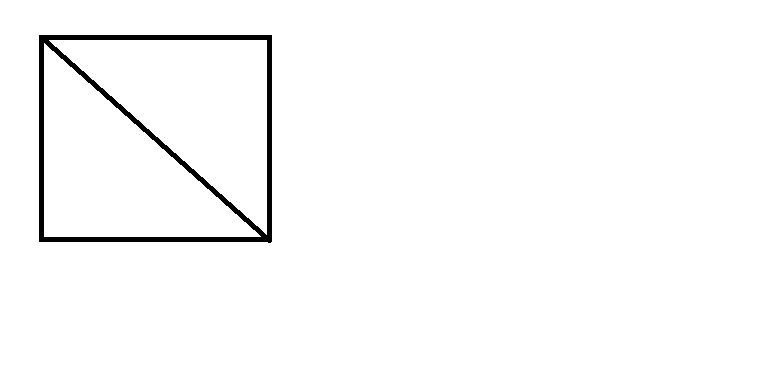
\includegraphics[width=\columnwidth]{graphics/reflection.png}	
	\caption{Reflection}
	\label{fig:Reflection}
\end{figure}

Dieser Ansatz und die Tatsache das wir diverse Probleme mit unserer statischen Multi-Window GUI hatten, haben uns dazu bewegt unser altes GUI-System abzulösen.
Dank unseren Properties war es uns mittels Reflection möglich ein neues dynamisches GUI System einzuführen, hierbei verzichteten wir auch auf das Multi-Window System und haben die GUI direkt auf den Sandkasten projeziert.


\clearpage
%% End Of Doc